\label{key}\documentclass[letterpaper, 12pt,oneside]{article}
\usepackage{amsmath}
\usepackage{graphicx}
\usepackage{xcolor}
\graphicspath{{Imagenes/}}
\usepackage[utf8]{inputenc}
\usepackage{listings}
\usepackage[hidelinks]{hyperref}

\title{\Huge Taller de Herramientas Computacionales}
\author{Josué Artemio Hernández Rodríguez}
\date{24/Enero/2019}

\begin{document}
	\maketitle
	\begin{center}
		
\includegraphics[scale=0.7]{3.jpg}
	\end{center}

	\newpage
	
	\title{\huge \textit{Bitácora problema 8 }}\\

	Este problema calcula el numero factorial, lo hice con el condicional \textit{while n $>$ 1:} y con una f = 1, antes del \textit{while}, por que inicia con 1. si n es mayor a 1, entonces esa f cambia a multiplicarse por n números anteriores, es decir f *= n y n -= 1; y me regresa f.  La solución solo bastaba que le pidiera al usuario esa n, que es el numero a calcularle el factorial. 
	  
	 

	\begin{figure}[h]
		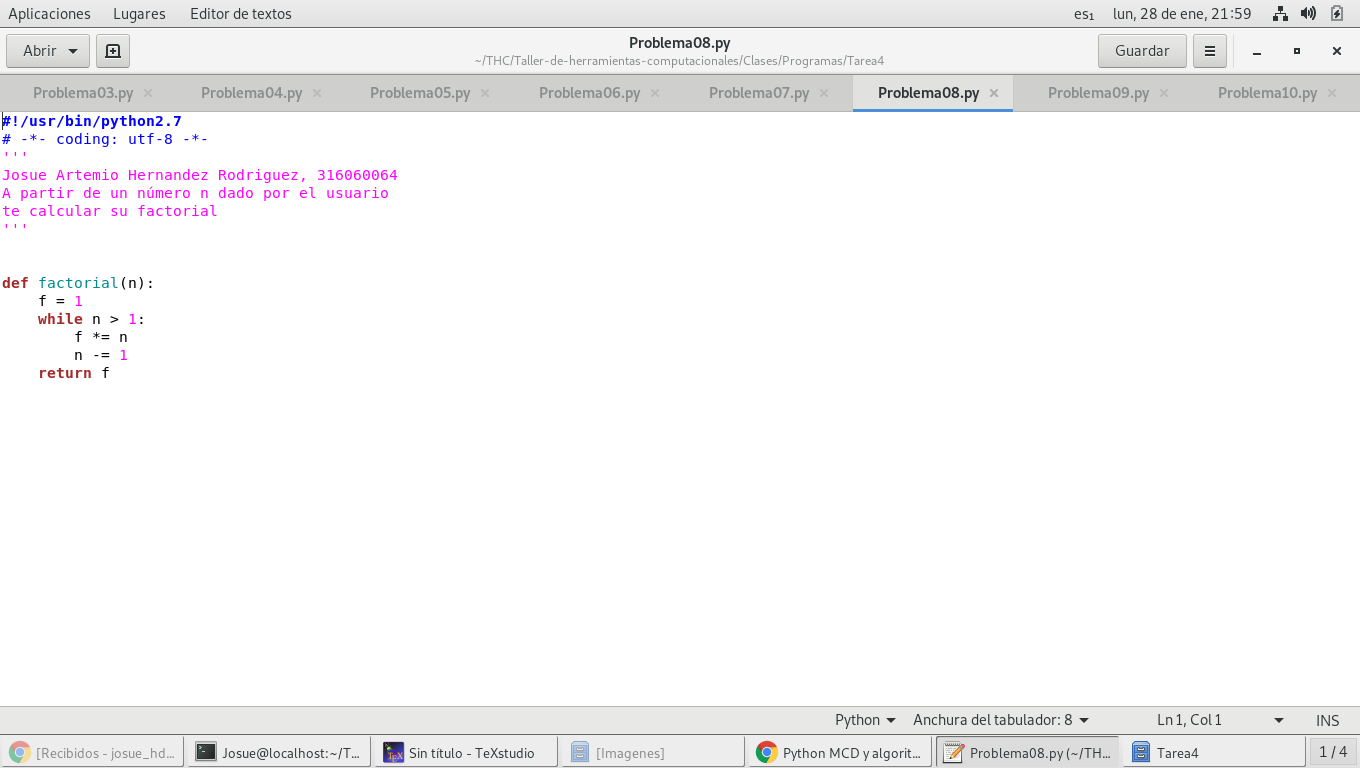
\includegraphics[scale=0.4]{pro08.png}
		
	\end{figure}

	
	
\end{document}
